\documentclass[twocolumn]{IEEEtran}
\usepackage{graphicx} % Required for inserting images
\usepackage{flushend}
\usepackage{float}
\usepackage{geometry}
\usepackage{amsmath}
\usepackage{subcaption}
\usepackage{booktabs} % For professional looking tables
\usepackage{setspace} % 设置行间距
\geometry{a4paper,scale=0.85}

\title{CW1 Lab Report}  
\author{Name: Junhao Huang \and Student ID: 2256793 \and TA: Yu Kang} 
\date{\today}  


\begin{document}
% \onehalfspacing  % 设置1.5倍行距

% 创建封面页
% \begin{titlepage}
%     \centering
%     \vspace*{3cm}
%     
\includegraphics[scale=1.2]{img/XJTLU.png}\\[1cm]
%     \vspace*{2cm}
%     \Large\textbf{CW1 Report}\\[1.0cm] % 文档标题
%     \normalsize Junhao Huang\\[0.2cm] % 作者名字
%     \normalsize INT104\\[0.2cm] % 机构名称
%     \normalsize \today % 日期
%     \vspace*{\fill} % 在页面底部添加垂直空间
% \end{titlepage}
\maketitle

% 介绍
\section{Introduction}
In this report, machine learning techniques are used to create a table of final exam information for the ICS program based on the information stored in the student performance information file provided. The table contains personally identifiable information of 619 students who participated in the final exam and the corresponding final exam grade information. In this paper, we will record a series of algorithms to validate the valid data in the data set and carry out data cleaning and preprocessing, and then filter the suitable feature set for data analysis according to the correlation between the data, and then downsize the data in the feature data set by using the PCA dimensional reduction algorithm to convert the high-dimensional data into a low-dimensional space, in order to obtain the visualization image that can reflect the distribution of the information about the students' grades as much as possible. Distribution of student achievement information as much as possible to get the visualization image.

% 数据分析
\section{Data Analysis}
% EDA
\subsection{Exploratory Data Analysis}
First of all, after the retrieval of the table, it can be seen that there is no duplication or missing content in the data in the table. So the data as a whole is clean and does not contain useless columns or rows. The original test scores can be analyzed according to the table below.
\begin{table}[htbp]
    \centering
    \caption{Summary Statistics of Exam Scores}
    \label{tab:exam_stats}
    \begin{tabular}{@{}lccc@{}}
    \toprule
    Feature & Max Value & Min Value & Average Value \\ \midrule
    Total   & 100       & 11        & 62.87         \\
    MCQ     & 54        & 6         & 34.58         \\
    Q1      & 8         & 0         & 6.67          \\
    Q2      & 8         & 0         & 3.82          \\
    Q3      & 14        & 0         & 10.76         \\
    Q4      & 10        & 0         & 5.84          \\
    Q5      & 6         & 0         & 1.19          \\ \bottomrule
    \end{tabular}
\end{table}
With respect to variability, the standard deviation indicates the degree to which scores differ, and the variability of the total score and MCQ is relatively high compared to the individual question scores. This scale change can skew the analysis, resulting in certain features having a disproportionate impact on the overall analysis. To mitigate this, subsequent consideration must be given to normalizing or standardizing the data to ensure that each feature contributes equally to subsequent analysis.

% 热力图
\subsection{HeatMap}
In order to gain a deeper understanding of the relationship between the elements. Combining the performance data in the table, the distribution of students' performance can be seen through the generated Fig. 1 to satisfy the Gaussian distribution, which is also known as the normal distribution. 
% 高斯分布
\begin{figure}[H]
    \centering % 使图片居中显示
    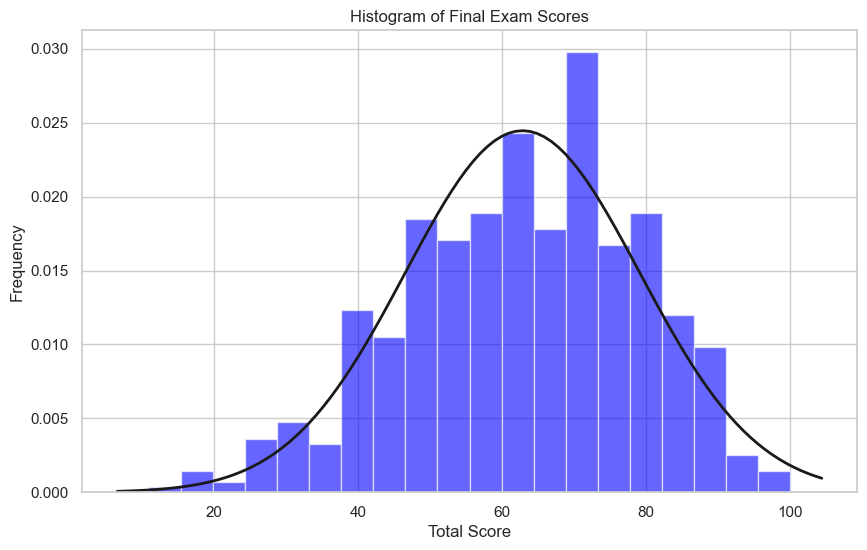
\includegraphics[scale=0.3]{./img/Gaussian.png}
    \caption{Take the Total feature in the data table to check whether the scores distribution of students in the final exam conforms to the Gaussian distribution}
\end{figure}
\vspace{-0.2cm}
When the Gaussian distribution is satisfied the Pearson algorithm can be used to find the correlation between the features, and the results can be generated by using the heatmap method in the seaborn library to generate a heat map for a clearer display of the correlation between the data. 
\vspace{-0.2cm}
% 热力图图像
\begin{figure}[H]
    \centering % 使图片居中显示
    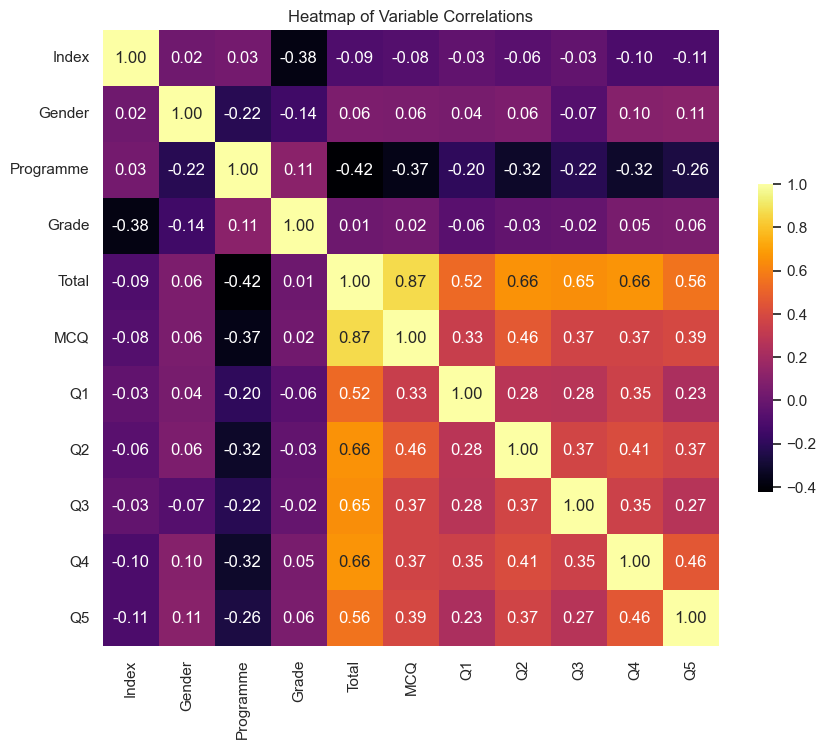
\includegraphics[scale=0.35]{./img/heatmap.png}
    \caption{Heatmap containing all the features, showing the correlation between the features by means of the Pearson algorithm. The warmer the color, the higher the positive correlation, and the colder the color, the higher the negative correlation.}
\end{figure}
\vspace{-0.2cm}
From the Fig. 2, it can be seen  that the correlation between Index, Gender and Grade is relatively small and weak for other features, where Index can be seen to have the least correlation with other features, so it can be removed first. Programme is negatively correlated, but negative correlation doesn't mean that it is not correlated, and at the same time, because the coursework uses the Programme features to act as a labeled feature set to divide the data, so Programme features can also be extracted.

% 随机森林
\subsection{Random Forest}
The final determination of whether Gender and Grade still need to be taken out can be done by using the Random Forest algorithm. 
\begin{equation}
    z = \frac{(x - \mu)}{\sigma}
\end{equation}
\textit{\(x\) is the original data point, \(\mu\) is the mean of the data set, \(\sigma\) is the standard deviation of the data set, and \(z\) is the standardized data point.} 

This can be done by using the RandomForestClassifier method in the sklearn library to show that the importance of each feature to the result can be assessed by analyzing the predictions produced by the decision tree constructed by the random forest algorithm. 
% 随机森林图像
\begin{figure}[H]
    \centering % 使图片居中显示
    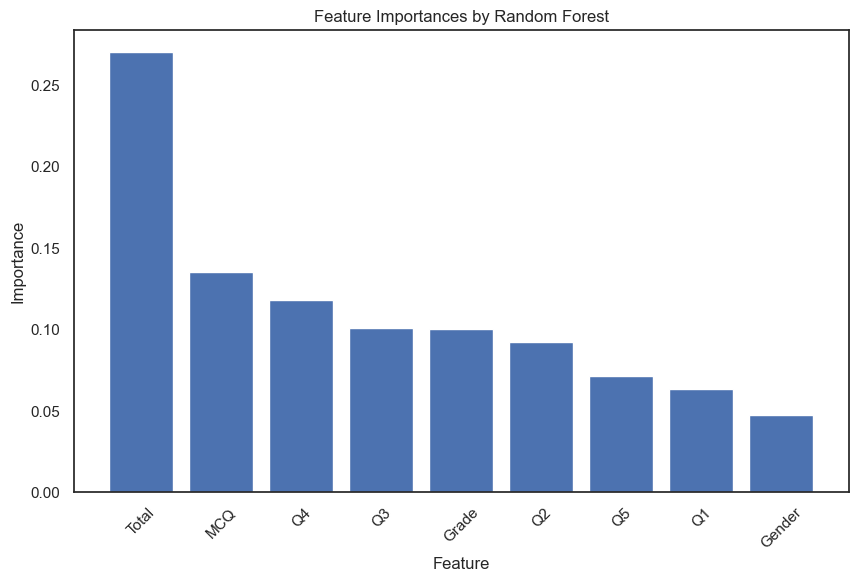
\includegraphics[scale=0.3]{./img/random_forest.png}
    \caption{The remaining 9 sets of features generate a histogram of the magnitude of the impact on the results}
\end{figure}
The Fig. 3 shows that the influence of Gender is minimized, so the removal of the Gender feature can also be considered.

% 标准化
\subsection{Standardization}
Principal component analysis is very sensitive to the scale of the feature data in the calculation process, so before the operation of principal component analysis, it is also necessary to standardize the selected data, by using the StandardScaler method in the sklearn library to standardize the current data, convert the data to a distribution with a mean of 0 and a standard deviation of 1 as the following Fig. 4 shows, from reducing the impact of the data differences on the accuracy of the the accuracy of the next operation.
% 标准化之后的图像
\begin{figure}[H]
    \centering % 使图片居中显示
    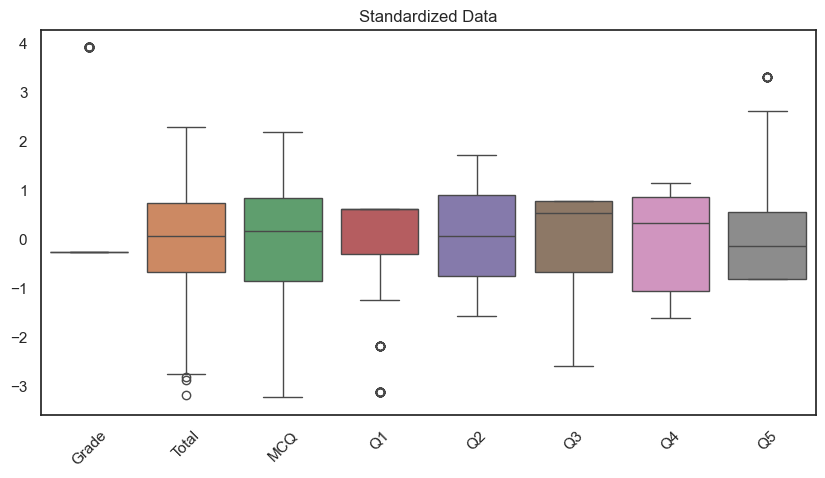
\includegraphics[scale=0.35]{./img/standard.png}
    \caption{A boxplot of the results obtained after standardizing the existing 8 sets of feature data}
\end{figure}

% 降维
\section{Dimensionality Reduction}
% 解释方差比
\subsection{Explained Variance Ratio}
Performing PCA dimensional reduction on the remaining feature dataset still retains relatively enough information to show the relationships between the original data.The basic idea of PCA is to reconstruct the n-dimensional feature set into k dimensions to generate new orthogonal features.The PCA operation selects the first principal component axes in the direction where the data has the largest variance, and the second principal component axes can be detected in the planes that are orthogonal to the first principal component axes. These new axes may show that most of the variance is contained in the first k axes, with less variance in the other axes. This is why only the first k axes containing most of the variance are retained as representative features of the data set. 
\begin{table}[H]
    \centering
    \begin{tabular}{@{}lccc@{}}
    \hline
    \textbf{Component} & \textbf{EVR (\%)} & \textbf{CVR (\%)} \\
    \hline
    1 & 46.59 & 46.59 \\
    2 & 12.96 & 59.54 \\
    3 & 9.59 & 69.13 \\
    4 & 9.43 & 78.56 \\
    5 & 8.19 & 86.76 \\
    6 & 7.06 & 93.82 \\
    7 & 6.17 & 99.99 \\
    8 & 0.006 & 100.00 \\
    \hline
    \end{tabular}
    \caption{Explained Variance Ratio(EVR) and Cumulative Variance Ratio (CVR) by PCA Components}
    \label{tab:pca_variance}
\end{table}
    
As shown in Table 2 for this dataset, based on the variance rates for all 8 axes, k was chosen as 2 because the majority of the variance is in the first and second axes.
% % PCA主成分占比
% \begin{figure}[H]
%     \centering
%     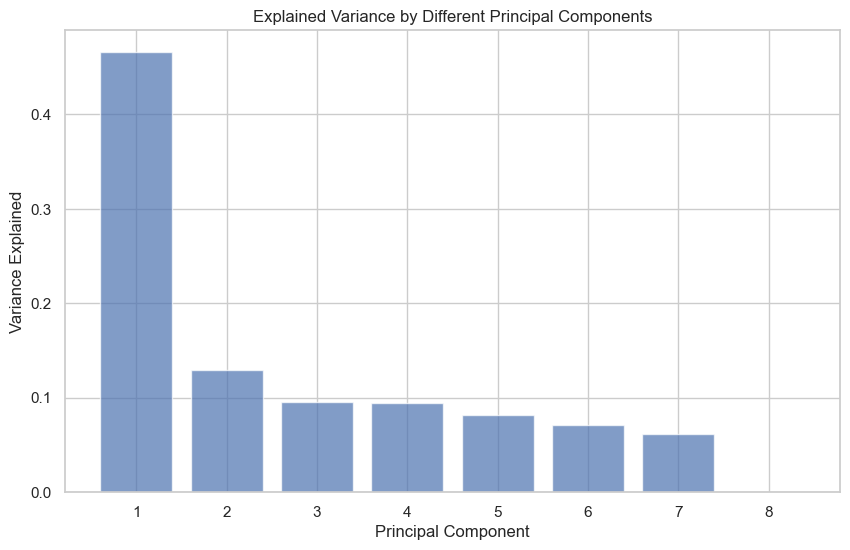
\includegraphics[scale=0.3]{./img/variance_count.png}
%     \caption{Variance Distribution}
% \end{figure}


% 累积方差比
\subsection{Cumulative Variance Ratio}
The cumulative explained variance ratio is used to show the ratio of the eigenvalues of the final selected principal component to the sum of all eigenvalues. Often if the ratio is higher, it indicates that the corresponding principal component captures more information
% \begin{figure}[H]
%     \centering
%     \includegraphics*[scale=0.3]{./img/cumulative.png}
%     \caption{shows how much information about the original data is retained with fewer principal components. The cumulative variance share in the graph is close to 1. If the cumulative variance share is high, it means that these principal components have captured most of the variability in the data.}
% \end{figure}
By calculating the cumulative explained variance ratios of the 8 principal components retained and finally presented on Table 2, the ratio of explained variance ratios is close to 1, implying that after reduce the dimensions of original data from 11 to 8, these principal components have captured most of the information about the data, and thus it can be finally confirmed that the table generated by the PCA performed through the 8 principal components can be chosen as the result of the final analysis.



% PCA公式
\subsection{Principal Component Analysis}
Calculate the covariance matrix of the data. If the data has n features, the covariance matrix will be an n-by-n matrix, where each element represents the covariance between pairs of response features. Covariance measures how two variables change together. For features X and Y, the covariance is calculated by:
\begin{equation}
    \text{Cov}(X, Y) = \frac{\sum_{i=1}^{n} (X_i - \bar{X})(Y_i - \bar{Y})}{n-1}
\end{equation}
\textit{where \(X\) and \(Y\) are the two variables, \(\bar{X}\) and \(\bar{Y}\) are their means, respectively, and \(n\) are the number of observations.}
    
% 接着,PCA通过特征分解协方差矩阵来计算:
\begin{equation}
    Cv = \lambda v
\end{equation}
\textit{where \(C\) is the covariance matrix, \(v\) is the eigenvector, and \(\lambda\) is the corresponding eigenvalue, representing the data variance in the \(v\) direction.}

% PCA图像
\begin{figure}[H]
    \centering
    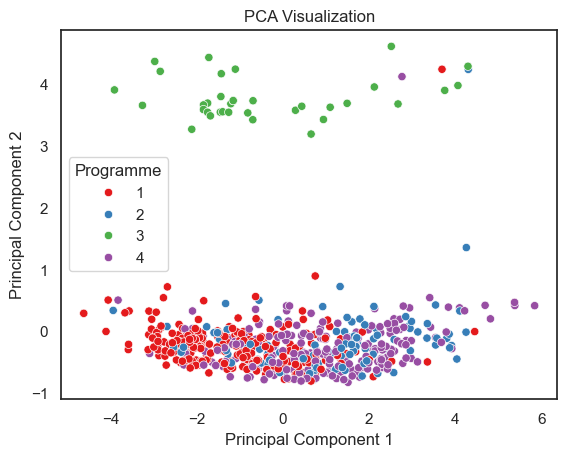
\includegraphics[scale=0.5]{./img/pca.png}
    \caption{Principal Component Analysis \(k=2\)}
\end{figure}
After the data preprocessing, the PCA method in sklearn library will be used to perform the computation, and the final result is shown in Fig. 5. The calculation of PCA requires the covariance matrix and the determination of the direction of the data. The covariance matrix will show the correlation between different features, and the largest two sets of eigenvalues can be found by eigendecomposition of the covariance matrix. The eigenvalues indicate the importance of the corresponding eigenvectors in the representation of principal components, so the corresponding principal components can be found according to the descending order of the eigenvalues, and the data will be mapped to the new coordinate system constructed by the principal components.

% tSNE降维
\subsection{tSNE}
In order to compare with the results obtained from the final PCA verification. Use the same data for tSNE method dimensionality reduction. tSNE is also a dimensionality reduction algorithm, but it is slightly different from PCA. PCA is a linear dimensionality reduction method that relies on the main direction of change of the data to reduce the dimensionality of the data, with a focus on preserving the global structure of the data. PCA, on the other hand, maps the data to a new coordinate system after orthogonal exchange.
% tSNE公式
\subsection*{t-SNE Target Function:}
\begin{equation}
    C = \sum_i \sum_j p_{ij} \log \frac{p_{ij}}{q_{ij}}.
\end{equation}
\textit{The cost function to be minimized, the sum of Kullback-Leibler divergences between \( p_{ij} \) which isHigher dimensional space and \( q_{ij} \) which is Lower dimensional space}

\begin{figure}[H]
    \centering
    \includegraphics*[scale=0.5]{./img/tsne.png}
    \caption{tSNE is a nonlinear dimensionality reduction technique that maps high-dimensional data to low-dimensional space by preserving the similarity between data points, and pays more attention to preserving the local structure of the data, making it easier to represent clusters or groups in high-dimensional data in low-dimensional space.}
\end{figure}
As can be seen from Fig. 6, tSNE provides a clearer separation and clustering of the student data for Program 3. However, the distribution of the remaining three majors is more aggregated on the second principal component and also has a certain positional distribution based on grades compared to the resulting image of PCA.
% 总结
\section{Conclusion}
There are two hypothesis based on result images. First, both PCA and tSNE basically separate Programme 3 students completely, and this may be because the vast majority of Programme 3 students are also Grade 3 students, which may be more relevant in themselves. Another piece of information is that the two students with full scores in this exam both appeared in Programme 1, while the lowest scores appeared in Programme 4. The distribution after dimensionality reduction can also roughly show that Programme 1 is distributed on the left and Programme 4 is distributed on the right.

\end{document}

